\documentclass[UTF8]{ctexart}
% 基本设置和必要宏包
\usepackage{geometry}
\geometry{a4paper,scale=0.8}

% 数学相关宏包
\usepackage{amsmath}
\usepackage{amssymb}
\usepackage{amsfonts}

\usepackage{mathtools}
\usepackage{amsbsy}
\usepackage{amstext}
\usepackage{wasysym}
\usepackage{stmaryrd}
\usepackage{mathrsfs}

% 图形和颜色
%\usepackage{xcolor}
\usepackage{graphicx}
\usepackage{subcaption}
\usepackage{caption}
\usepackage{float}

% 其他功能性宏包
\usepackage{titlesec}
\usepackage{fancyhdr}
\usepackage{setspace}
\usepackage{cite}
\usepackage{appendix}
\usepackage{listings}
\usepackage{pdfpages}
\usepackage{enumitem}
\usepackage{tabu}
\usepackage{threeparttable}
\usepackage{booktabs}
\usepackage{abstract}


\usepackage{diagbox} 

% 允许公式跨页
\allowdisplaybreaks[4]



\newcommand{\sihaoheiti}{\fontsize{14pt}\selectfont\heiti}
% 设置全局字体
%\setCJKmainfont{SimSun} % 设置正文为宋体
%\setCJKsansfont{SimHei} % 设置无衬线字体为黑体

% 论文题目设置为三号黑体字,并居中
\newcommand{\threelargebf}{\fontsize{16pt}{19.2pt}\selectfont\heiti\centering}

% 一级标题设置为四号黑体字,并居中
\titleformat{\section}{\centering\fontsize{14pt}{16pt}\bfseries\heiti}{\thesection}{1em}{}

% 二级标题设置为小四号黑体字,左对齐
\titleformat{\subsection}{\fontsize{12pt}{14.4pt}\bfseries\heiti}{\thesubsection}{1em}{\raggedright}

% 三级标题设置为小四号黑体字,左对齐
\titleformat{\subsubsection}{\fontsize{12pt}{14.4pt}\bfseries\heiti}{\thesubsubsection}{1em}{\raggedright}

% 正文字体设置为小四号宋体字,并使用单倍行距
\renewcommand{\normalsize}{\fontsize{12pt}{14.4pt}\selectfont}
%\renewcommand{\baselinestretch}{3}
%\selectfont



%\linespread{5.0}%修改行距
\graphicspath{{img/}}
\let\itemize\compactitem
\let\enditemize\endcompactitem
% 设置页面布局
\geometry{a4paper, left=2.5cm, right=2.5cm, top=3cm, bottom=3cm}
\setstretch{2}

\renewcommand{\arraystretch}{1.5}
\newcommand{\thickhline}{\noalign{\hrule height 1.2pt}} % 设置粗线的宽度
\newcommand{\thinhline}{\noalign{\hrule height 0.8pt}} % 设置细线的宽度

%%%% ===== 定理环境
\usepackage[amsmath,thref,thmmarks,hyperref]{ntheorem} % 定理宏包
%\theorempreskipamount1em % spacing before the environment
%\theorempostskipamount0em  % spacing after the environment
%\theoremstyle{plain}
%\theoremheaderfont{\normalfont\heiti}
%\theorembodyfont{\normalfont\kaishu}
%\theoremindent0em
%\theoremseparator{\hspace{0.2em}}
%\theoremnumbering{arabic}

\newtheorem{property}{性质}[section]
\newtheorem{definition}{定义}[section]
\newtheorem{lemma}{引理}[section]
\newtheorem{remark}{注记}[section]
\newtheorem{corollary}{推论}[section]
\newtheorem{example}{例}[section] 
\newtheorem{problem}{{问题}}

 \renewcommand{\abstractnamefont}{\normalfont\bfseries}  % 摘要标题字体:正常字体,粗体
\renewcommand{\abstracttextfont}{\normalfont\normalsize}     % 摘要内容字体:正常字体,小四号

% 设置页眉页脚
\pagestyle{fancy}
\fancyhf{}
\fancyfoot[C]{\thepage}
\renewcommand{\headrulewidth}{0pt}

% 设置标题格式
\titleformat{\section}{\centering\heiti\large}{\thesection}{1em}{}
\titleformat{\subsection}{\raggedright\heiti\normalsize}{\thesubsection}{1em}{}
\titleformat{\subsubsection}{\raggedright\heiti\normalsize}{\thesubsubsection}{1em}{}

% 设置摘要环境
%\newenvironment{myabstract}{
%	\begin{center}
%	\bfseries\zihao{-3} 摘要
%	\end{center}
%	\vspace{-0.5em} % 调整摘要与论文题目的距离
%	\normalsize
%}{
%}
% 设置附录环境
\renewcommand{\appendixname}{附录}
\renewcommand{\appendixpagename}{附录}

% 设置代码环境
\lstset{
	basicstyle=\small\ttfamily,
	keywordstyle=\color{blue},
	commentstyle=\color{green!70!black},
	stringstyle=\color{red},
	breaklines=true,
	numbers=left,
	numberstyle=\tiny,
	frame=tb,
	language=Python
}
\newcommand{\bbA}{\mathbb{A}}
\newcommand{\bbB}{\mathbb{B}}
\newcommand{\bbC}{\mathbb{C}}
\newcommand{\bbD}{\mathbb{D}}
\newcommand{\bbE}{\mathbb{E}}
\newcommand{\bbF}{\mathbb{F}}
\newcommand{\bbG}{\mathbb{G}}
\newcommand{\bbH}{\mathbb{H}}
\newcommand{\bbI}{\mathbb{I}}
\newcommand{\bbJ}{\mathbb{J}}
\newcommand{\bbK}{\mathbb{K}}
\newcommand{\bbL}{\mathbb{L}}
\newcommand{\bbM}{\mathbb{M}}
\newcommand{\bbN}{\mathbb{N}}
\newcommand{\bbO}{\mathbb{O}}
\newcommand{\bbP}{\mathbb{P}}
\newcommand{\bbQ}{\mathbb{Q}}
\newcommand{\bbR}{\mathbb{R}}
\newcommand{\bbS}{\mathbb{S}}
\newcommand{\bbT}{\mathbb{T}}
\newcommand{\bbU}{\mathbb{U}}
\newcommand{\bbV}{\mathbb{V}}
\newcommand{\bbW}{\mathbb{W}}
\newcommand{\bbX}{\mathbb{X}}
\newcommand{\bbY}{\mathbb{Y}}
\newcommand{\bbZ}{\mathbb{Z}}

\title{}
\author{}
\date{}

\begin{document}

\begin{titlepage}		
	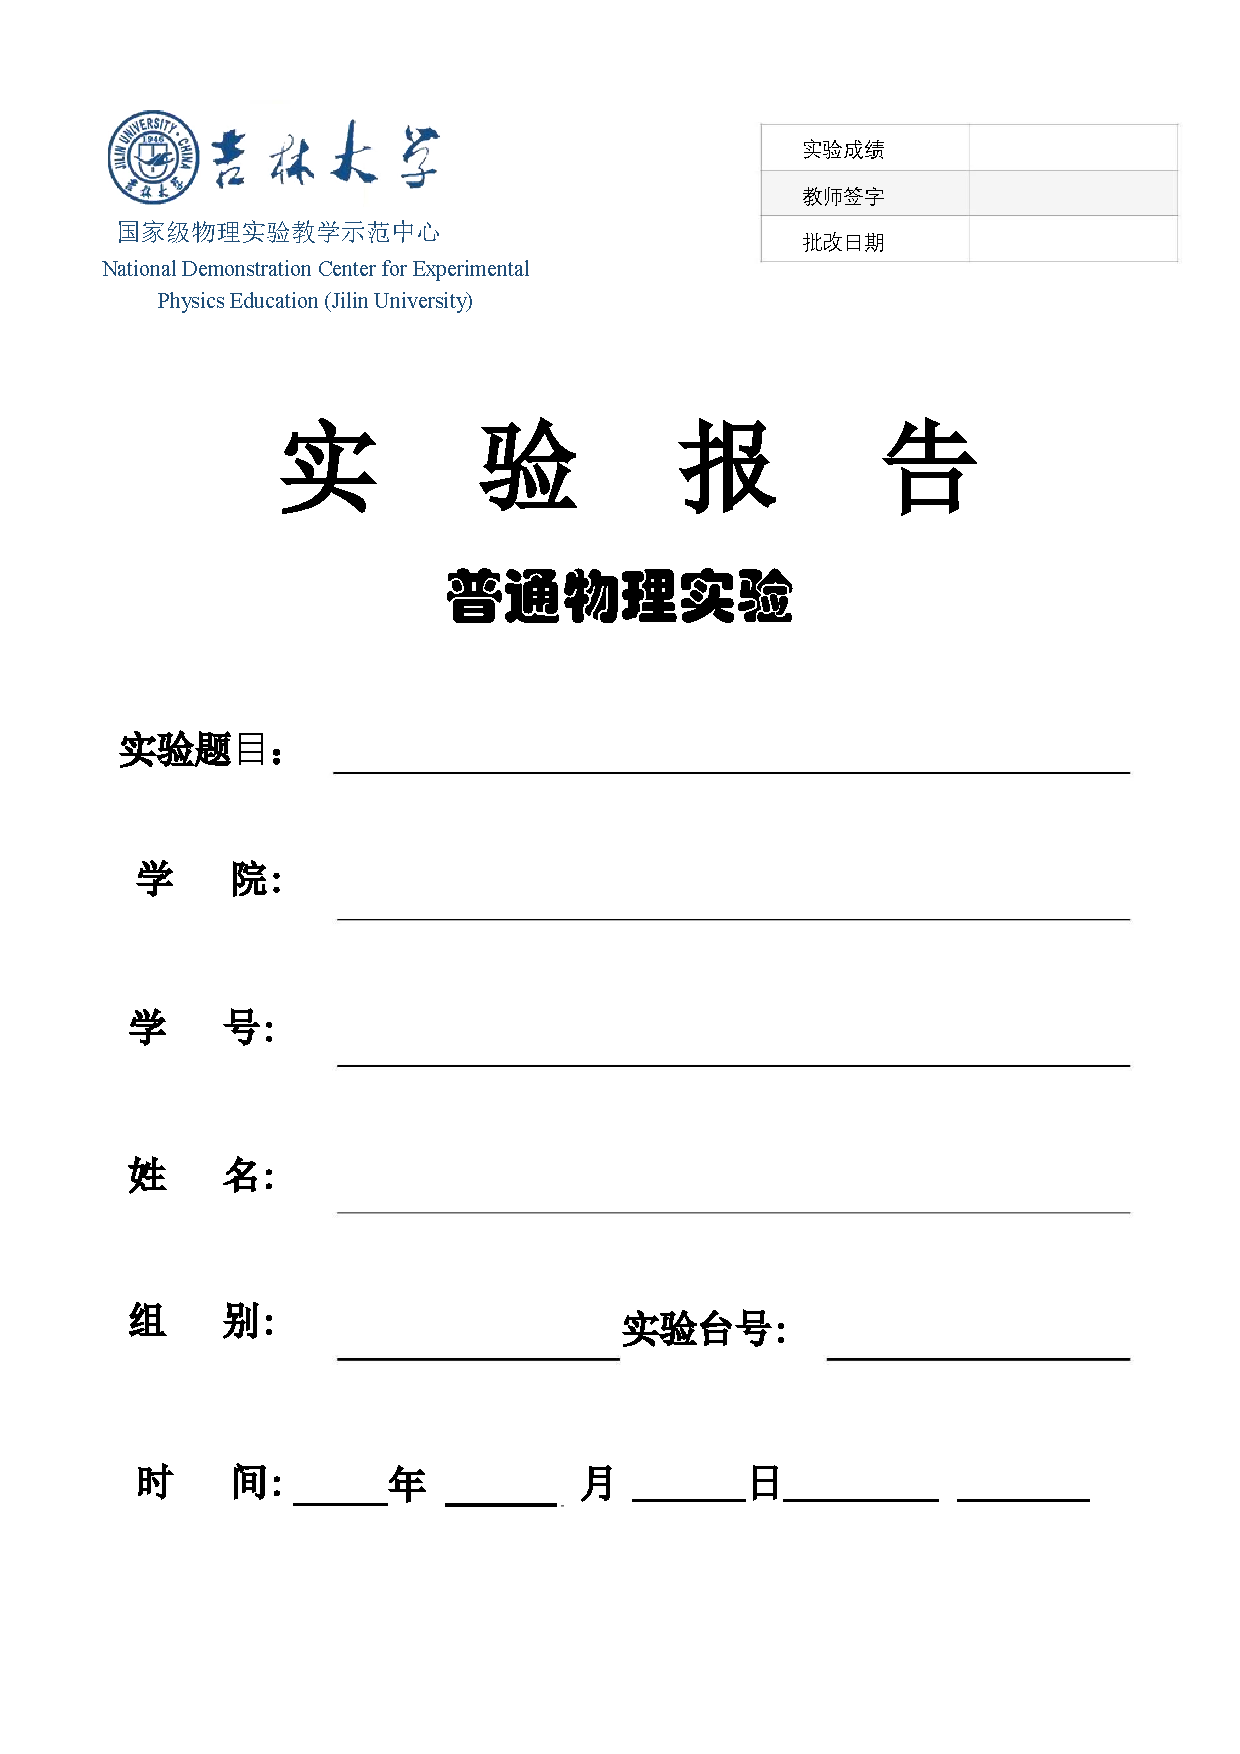
\includepdf[pages=-]{封面.pdf}
\end{titlepage}


\section{实验内容}
\setstretch{0.9}
\begin{enumerate}
    \item 记录游标卡尺、螺旋测微器、计数显微镜的量程和精度,物理天平的量程和分度值。
    \item 用游标卡尺测量圆柱的高度 $h$,细线长度 $l$,测量三次。
    \item 用螺旋测尾气测量圆柱的直径 $D_1$ 、圆球的直径 $D_2$ ,测量六次。
    \item 用读数显微镜测量细线物品的直径 $D_3$,测量六次。
    \item 用物理天平测量圆柱和圆球的质量 $m_1$ 和 $m_2$,测量三次。用电子天平测量细线质量 $m_3$,测量一次。
    \item 计算圆柱,圆球和细线的密度 $\rho$:
    $$\rho_{\text{圆柱}} = \frac{4m_1}{\pi D_1^2 h},\  \rho_{\text{圆球}} = \frac{6m_2}{\pi D_2^3},\  \rho_{\text{细线}} = \frac{4m_3}{\pi D_3^2l}$$
\end{enumerate}

\section{原始数据}
\begin{table}[H]
\centering
\caption{量程和精度数据}
\begin{tabular}{|c|c|c|c|c|c|}
\hline
     & 游标卡尺 & 螺旋测微器 & 读数显微镜  & 物理天平  & 电子天平 \\
\hline
     量程 &  $0\sim 200mm$ & $0 \sim 25mm$ & $0 \sim 50mm$  & $0 \sim 500g$ & $0 \sim 150g$ \\
\hline 
    精度  & 0.02mm &  0.01mm & 0.01mm & (分度值)50mg  & 0.0001g\\
\hline
\end{tabular}
\end{table}

\begin{table}[H]
\centering
\caption{游标卡尺测量圆柱高度、细线物品长度}
\begin{tabular}{|c|c|c|c|}
\hline
     测量次数 & 1 & 2 & 3  \\
\hline
     圆柱高度$h/mm$ & 29.32 & 29.34 & 29.32 \\ 
\hline
     细线物品长度 $l/mm$ & 113.48 & 113.50 & 113.50\\ 
\hline
\end{tabular}
\end{table}

\begin{table}[H]
\centering
\caption{螺旋测微器测量圆柱与圆球的直径}
\begin{tabular}{|c|c|c|c|c|c|c|}
\hline
     测量次数 & 1 & 2 & 3 & 4 & 5 & 6 \\
\hline
     圆柱的直径 $D_1$/mm & 9.985 & 9.980 & 9.983 & 9.990 & 9.986 & 9.985 \\ 
\hline
     圆球的直径 $D_2$/mm & 10.989 & 10.990 & 10.991 &  10.990 & 10.991 & 10.991\\ 
\hline
\end{tabular}
\end{table}

\begin{table}[H]
\centering
\caption{读数显微镜测量细线物品的直径}
\begin{tabular}{|c|c|c|c|c|c|c|}
\hline
     测量次数 & 1 & 2 & 3 & 4 & 5 & 6 \\
\hline
    细线物品的直径$D_3$ & 0.563 & 0.576 & 0.574 & 0.569 & 0.578 & 0.577 \\
\hline
\end{tabular}
\end{table}

\begin{table}[H]
\centering
\caption{物理天平测量圆柱和圆球的质量}
\begin{tabular}{|c|c|c|c|}
\hline
     测量次数 & 1 & 2 & 3  \\
\hline
     圆柱质量$m_1/g$ & 17.97 & 17.96 & 17.98 \\ 
\hline
     圆球质量 $m_2/g$ & 5.50 & 5.48 & 5.50\\ 
\hline
\end{tabular}
\end{table}
电子天平测量细线物品的质量,测一次得到细线物品的质量 $m_3$ 为:$0.2487g$

\section{数据处理}
\subsection{数据平均值与不确定度的计算}
\subsubsection{数据平均值的计算}
根据 $\S 2$ 中表格计算出 $h$、$D_2$、$D_2$、$D_3$、$l$、$m_1$、$m_2$ 的平均值如下:
\begin{align*}
    \overline{h} &= \frac{\sum_{i=1}^3 h_i}{3} = \frac{29.32+29.34+29.32}{3} mm = 29.33 mm\\
    \overline{l} &= \frac{\sum_{i=1}^3 l_i}{3} = \frac{113.48+113.50+113.50}{3} mm = 113.49 mm \\
    \overline{D_1} &= \frac{\sum_{i=1}^6 D_1^i}{6} = \frac{9.985+9.980+9.983+9.990+9.986+9.985}{6} mm = 9.985 mm\\
    \overline{D_2} &= \frac{\sum_{i=1}^6 D_2^i}{6} = \frac{10.989+10.990+10.991+10.990+10.991+10.991}{6} mm = 10.990 mm\\
    \overline{D_3} &= \frac{\sum_{i=1}^6 D_3^i}{6}  =  \frac{0.563+0.576+0.574+0.569+0.578+0.577}{6} mm =  0.573mm\\
    \overline{m_1} &= \frac{\sum_{i=1}^3 m_1^i}{3} = \frac{17.97+17.96+17.98}{3}  g=  17.97g\\
    \overline{m_2} &= \frac{\sum_{i=1}^3 m_2^i}{3} = \frac{5.50+5.48+5.50}{3}g  =  5.49g\\
\end{align*}

\begin{table}[H]
\centering
\caption*{测量数据的平均值}
\begin{tabular}{c c c c c c c c}
\toprule[1pt]
\midrule
     测量指标 & $\overline{h}$ & $\overline{l}$ & $\overline{D_1}$ & $\overline{D_2}$ & $\overline{D_3}$ & $\overline{m_1}$ & $\overline{m_2}$  \\
\midrule
     数据 & 29.33mm& 113.49mm& 9.985mm & 10.990mm&0.573mm & 17.97g  &5.49g\\
\midrule
\bottomrule[1pt]
\end{tabular}
\end{table}

\subsubsection{数据不确定度的计算}

\begin{spacing}{1.2}
\textbf{一.合成不确定度}

设 $u_A(o)$、$u_B(o)$、$u_c(o)$ 分别为测量指标 $o$ 由统计方法得到的 $A$ 类标准不确定度,仪器允差带来的不确定度分量 $B$,以及按方和根方法合成的标准不确定度$C$。假设得到的不确定度分量相互独立。
$$
u_A(o) = \sqrt{\frac{\sum_{i=1}^n (o_i - \overline{o})^2}{n\times (n-1)}}
$$

假设误差为均匀分布则得到 
\end{spacing}

\begin{align*}
    u_B(o) &= \frac{o_{\text{仪器误差}}}{\sqrt{3}} \\
    u_c(o) &= \sqrt{u_A(o)^2+u_B(o)^2}
\end{align*}


\begin{spacing}{1.35}
\textbf{(1) A类标准不确定度的计算}


根据上述给出的 $A$ 类标准不确定度的计算公式
\end{spacing}

$$u_A(o) = \sqrt{\frac{\sum_{i=1}^n (o_i - \overline{o})^2}{n\times (n-1)}}$$

代入上表中数据求得各数据 $A$ 类标准不确定度如下:

   \begin{align*}
      u_{A}(h)  &= \sqrt{\frac{\sum_{i=1}^{3}(h_i-\overline{h})^2}{3\times 2}} =  \sqrt{\frac{(29.32-29.33)^2 +\cdots + (29.32-29.33)^2}{6}} mm  = 0.007mm
      \\
      u_A(l)  &= \sqrt{\frac{\sum_{i=1}^{3}(l_i-\overline{l})^2}{3\times 2}} = 
      \sqrt{\frac{(113.48-113.49)^2 + \cdots + (113.50-113.49)^2}{6}} mm = 0.007 mm
      \\
      u_A(D_1) &= \sqrt{\frac{\sum_{i=1}^{6}(D_1^i-\overline{D_1})^2}{6\times 5}} = \sqrt{\frac{(9.985-9.985)^2 + \cdots + (9.985-9.985)^2}{30}mm} = 0.0014mm\\
      u_A(D_2) &= \sqrt{\frac{\sum_{i=1}^{6}(D_2^i-\overline{D_2})^2}{6\times 5}}  = \sqrt{\frac{(10.989 - 10.990)^2+ \cdots + (10.991-10.990)^2}{30}} mm = 0.0004mm
      \\
      u_A(D_3) &= \sqrt{\frac{\sum_{i=1}^{6}(D_3^i-\overline{D_3})^2}{6\times 5}}  = \sqrt{\frac{(0.563-0.573)^2 + \cdots + (0.577-0.573)^2}{30}}mm = 0.0024mm\\
      u_A(m_1) & = \sqrt{\frac{\sum_{i=1}^{3}(m_1^i-\overline{m_1})^2}{3\times 2}}  = \sqrt{\frac{(17.97-17.97)^2 + (17.96-17.97)^2 + (17.98-17.97)^2}{6}}mm  \\ &= 0.0058mm\\
      u_A(m_2) & = \sqrt{\frac{\sum_{i=1}^{3}(m_2^i-\overline{m_2})^2}{3\times 2} } = \sqrt{\frac{(5.50-5.49)^2 + (5.48-5.49)^2 + (5.50-5.49)^2}{6}} mm  \\ &= 0.007  mm\\
      u_A(m_3) & = \sqrt{\frac{\sum_{i=1}^{1}(m_3^i-\overline{m_3})^2}{1\times 1}} mm = 0 mm\\
   \end{align*}

   
\newpage

\begin{spacing}{1.35}
\textbf{(2) B类不确定度的计算}

根据上述 $B$ 类不确定度的公式 

$$u_B(o) = \frac{o_{\text{仪器误差}}}{\sqrt{3}}$$

代入上述表中数据可得
\end{spacing}


\begin{align*}
 u_{B}(h)  &= \frac{\Delta h_{\text{仪器误差}}}{\sqrt{3}}   = 0.012 mm\\
      u_B(l)  &= \frac{\Delta l_{\text{仪器误差}}}{\sqrt{3}} mm  = 0.012 mm\\
      u_B(D_1) &= \frac{\Delta D_{1_{{\text{仪器误差}}}}}{\sqrt{3}} mm=  0.006 mm\\
      u_B(D_2) &= \frac{\Delta D_{2_{{\text{仪器误差}}}}}{\sqrt{3}}mm =0.006 mm \\
      u_B(D_3) &= \frac{\Delta D_{3_{{\text{仪器误差}}}}}{\sqrt{3}} mm= 0.006 mm\\
      u_B(m_1) & = \frac{\Delta m_{1_{{\text{仪器误差}}}}}{\sqrt{3}} mm = 0.03mm\\
      u_B(m_2) & =\frac{\Delta m_{2_{{\text{仪器误差}}}}}{\sqrt{3}} mm = 0.03 mm\\
      u_B(m_3) & =\frac{\Delta m_{3_{{\text{仪器误差}}}}}{\sqrt{3}} mm= 0.00006 mm
      \\
\end{align*}

\textbf{(3) 合成标准不确定度的计算}

\begin{align*}
    u_c(h) &= \sqrt{u_A(h)^2+u_B(h)^2}  = \sqrt{\frac{\sum_{i=1}^{3}(h_i-\overline{h})^2}{3\times 2}+\frac{\Delta^2h_{\text{仪器误差}}}{3}} = \sqrt{(0.007)^2+(0.012)^2}mm =0.014 mm\\
    u_c(l) &= \sqrt{u_A(l)^2+u_B(l)^2}  = \sqrt{\frac{\sum_{i=1}^{3}(l_i-\overline{l})^2}{3\times 2}+\frac{\Delta^2l_{\text{仪器误差}}}{3}} = \sqrt{(0.007)^2+(0.012)^2}mm =0.014 mm\\
    u_c(D_1) &= \sqrt{u_A(D_1)^2+u_B(D_1)^2}  = \sqrt{\frac{\sum_{i=1}^{6}(D_1^i-\overline{D_1})^2}{6\times 5}+\frac{\Delta^2D_{1_{{\text{仪器误差}}}}}{3}} \\&= \sqrt{(0.0014)^2+(0.006)^2}mm = 0.0062 mm\\
    u_c(D_2) &= \sqrt{u_A(D_2)^2+u_B(D_2)^2}  = \sqrt{\frac{\sum_{i=1}^{6}(D_2^i-\overline{D_2})^2}{6\times 5}+\frac{\Delta^2D_{2_{{\text{仪器误差}}}}}{3}} \\&= \sqrt{(0.0004)^2+(0.006)^2}mm = 0.0060  mm \\
    u_c(D_3) &= \sqrt{u_A(D_3)^2+u_B(D_3)^2}  = \sqrt{\frac{\sum_{i=1}^{6}(D_3^i-\overline{D_3})^2}{6\times 5}+\frac{\Delta^2D_{3_{{\text{仪器误差}}}}}{3}} \\&= \sqrt{0.0024)^2+(0.006)^2}mm = 0.0065mm\\
    u_c(m_1) &= \sqrt{u_A(m_1)^2+u_B(m_1)^2}  = \sqrt{\frac{\sum_{i=1}^{3}(m_1^i-\overline{m_1})^2}{3\times 2}+\frac{\Delta^2 m_{1_{{\text{仪器误差}}}}}{3}} \\&= \sqrt{(0.0058)^2+(0.03)^2}mm = 0.031mm \\
    u_c(m_2) &= \sqrt{u_A(m_2)^2+u_B(m_2)^2}  = \sqrt{\frac{\sum_{i=1}^{3}(m_2^i-\overline{m_2})^2}{3\times 2}+\frac{\Delta^2 m_{2_{{\text{仪器误差}}}}}{3}} \\&= \sqrt{(0.007)^2+(0.03)^2}mm = 0.031mm \\
    u_c(m_3) &= \sqrt{u_A(m_3)^2+u_B(m_3)^2}  = \sqrt{\frac{\sum_{i=1}^{1}(m_3^i-\overline{m_3})^2}{1}+\frac{\Delta^2 m_{3_{{\text{仪器误差}}}}}{3}}  \\&= \sqrt{0+(0.00006)^2}mm = 0.00006mm\\
\end{align*}

\begin{spacing}{1.2}
\textbf{(4)扩展不确定度的计算以及相对不确定度的计算}

扩展不确定度 $U_{i} = k_p u_{c}(i)$,其中根据正态分布置信概率 $K_p$ 与 $p$的关系如下表可知
\end{spacing}
\begin{table}[H]
\centering
\begin{tabular}{|c|c|c|c|c|c|c|c|}
\hline
     p & $0.500$ & $0.683$ & $0.900$ & $0.950$ & $0.955$ & $0.990$ & $0.997$  \\
\hline
      $K_p$ & $0.675$ & $1$ & $1.65$ & $1.96$ & $2$ & $2.58$ & $3$ \\
\hline
\end{tabular}
\caption*{}
\end{table}

\begin{spacing}{1.2}
    代入 $p=0.950$ 时 $K_{0.950} = 1.96$ 的置信概率得到$h$、$D_2$、$D_2$、$D_3$、$l$、$m_1$、$m_2$、$m_3$ 的扩展不确定度如下
\end{spacing}

\begin{align*}
  U_{h} &= K_{0.950} \times u_c(h) = 1.96 \times 0.014mm = 0.027 mm  \\
  U_{l} &= K_{0.950} \times u_c(l) = 1.96 \times0.014 mm =  0.027mm \\
  U_{D_1} &= K_{0.950} \times u_c(D_1) = 1.96 \times 0.0062 mm = 0.0122 mm \\
  U_{D_2} &= K_{0.950} \times u_c(D_2) = 1.96 \times 0.0060 mm = 0.0118 mm \\
  U_{D_3} &= K_{0.950} \times u_c(D_3) = 1.96 \times 0.0065  mm = 0.0127 mm \\
  U_{m_1} &= K_{0.950} \times u_c(m_1) =1.96 \times 0.031 mm = 0.061 mm  \\
  U_{m_2} &= K_{0.950} \times u_c(m_2) = 1.96 \times 0.031 mm = 0.061 mm  \\
  U_{m_3} &= K_{0.950} \times u_c(m_3) = 1.96 \times 0.00006 mm = 0.00012  mm 
\end{align*}

由相对不确定度公式

$$E(i) = \frac{u_c(i)}{\overline{i}} \times 100\% $$

代入上述得到数据可计算相对不确定度如下:

\begin{align*}
    E(h) &= \frac{u_c(h)}{\overline{h}} \times 100\% = \frac{0.014}{29.33} \times 100 \% = 0.05\%\\
    E(l) &= \frac{u_c(l)}{\overline{l}} \times 100\% = \frac{0.014}{113.49} \times 100 \% =0.01\%\\
    E(D_1) &= \frac{u_c(D_1)}{\overline{D_1}} \times 100\% = \frac{0.0062}{9.985} \times 100 \% =0.06\%\\
    E(D_2) &= \frac{u_c(D_2)}{\overline{D_2}} \times 100\% = \frac{0.0060}{10.990} \times 100 \% =0.05\%\\
    E(D_3) &= \frac{u_c(D_3)}{\overline{D_3}} \times 100\% = \frac{0.0065}{0.573} \times 100 \% =1.13\%\\
    E(m_1) &= \frac{u_c(m_1)}{\overline{m_1}} \times 100\% = \frac{0.031}{17.97} \times 100 \% =0.17\%\\
    E(m_2) &= \frac{u_c(m_2)}{\overline{m_2}} \times 100\% = \frac{0.031}{5.49} \times 100 \% =0.56\%\\
    E(m_3) &= \frac{u_c(m_3)}{m_3} \times 100\% = \frac{0.00006}{0.2487} \times 100 \% =0.02\%\\
\end{align*}

\begin{table}[H]
\centering
\caption*{测量数据}
\begin{tabular}{c|c|c|c|c|c|c|c}
\toprule[1pt]
\midrule
     计算指标 & $\overline{i}$ & $u_A(i)$ & $u_B(i)$ & $u_{c}(i)$ & $U(i)$ & $E(i)$  & $i=\overline{i} \pm U(i)$ \\
\midrule
      圆柱高度$h$&29.33  & 0.007 & 0.012 & 0.014 & 0.027 & $0.05\%$ &  $29.33 \pm 0.027$  \\
\midrule
细线长度$l$& 113.49 & 0.007 & 0.012 & 0.014& 0.027 & $0.01\%$&  $113.49 \pm 0.027$   \\
\midrule
圆柱直径$D_1$&9.985  & 0.0014 & 0.006 &0.0062 & 0.0122 & $0.06\%$ &  $9.985 \pm 0.0122$   \\
\midrule
圆球直径$D_2$& 10.990 & 0.0004 & 0.006 & 0.0060& 0.0118 & $0.05\%$ &  $0.990 \pm 0.0118$   \\
\midrule
细线直径$D_3$& 0.573 & 0.0023 & 0.006& 0.0065 & 0.0127 &$1.13\%$  &  $0.573 \pm 0.0127$   \\
\midrule
圆柱质量$m_1$& 17.97 & 0.0058 & 0.03 & 0.031 & 0.061 & $0.17\%$  & $17.97 \pm 0.061$ \\
\midrule
圆球质量$m_2$&5.49  & 0.007 & 0.03 & 0.031 & 0.061 & $0.56\%$ &  $5.49 \pm 0.061$   \\
\midrule
细线质量$m_3$& 0.2487 & 0 & 0.00006 & 0.00006 & 0.00012 &  $0.02\%$ & $0.2487 \pm 0.00012$ \\
\midrule
\bottomrule[1pt]
\end{tabular}
\end{table}


\begin{spacing}{1.2}
由表格幅度所限,故上述表格未展示数据的单位,现在此处标明:

圆柱高度$h$、细线长度$l$、圆柱直径$D_1$、圆球直径$D_2$、细线直径$D_3$ 以及其所代表的$\overline{i}$、 $u_A(i)$、$u_B(i)$、$u_{c}(i)$、$U(i)$、$i=\overline{i} \pm U(i)$ 单位均为 $mm$

而圆柱质量$m_1$、圆球质量$m_2$、细线质量$m_3$ 及其所代表的$\overline{i}$、 $u_A(i)$、$u_B(i)$、$u_{c}(i)$、$U(i)$、$i=\overline{i} \pm U(i)$ 单位均为 $g$
\end{spacing}






\subsection{计算各样品的密度及其扩展不确定度的}
\subsubsection{计算各样品密度}
\begin{align*}
    \rho_{\text{圆柱}} &= \frac{4m_1}{\pi D_1^2 h} = \frac{4 \times 17.97}{ \pi \times 9.985^2 \times 29.33} \ g/mm^3 =  7.824 g/cm^3\\
    \rho_{\text{圆球}} &= \frac{6m_2}{\pi D_2^3} = \frac{6 \times 5.49 }{\pi \times 10.990^3 } \ g/mm^3= 7.899 g/cm^3\\
    \rho_{\text{细线}} &= \frac{4m_3}{\pi D_3^2l} = \frac{4 \times 0.2487 }{\pi \times 0.573^2 \times 113.49 } \ g/mm^3 =8.498g/cm^3
\end{align*}

\subsubsection{计算标准不确定度}
由标准的不确定度传递公式 
\begin{align*}
    y &= f(x_1,x_2,\dots,x_n) \\
    u_c(y) &= \sqrt{\sum_{i=1}^{n}(\frac{\partial f}{\partial x_i})^2 u^2_{c(x_i)}}
\end{align*}

又由原题目中给出的圆柱的标准不确定度的公式如下:

\begin{align*}
\frac{u_{\rho(\text{圆柱})}}{\rho_{\text{圆柱}}} &=  \sqrt{
\Big( \frac{\partial \rho_{\text{圆柱}} } {\partial m_1} \Big)^2 \frac{u^2_{c(m_1)}}{\rho_{\text{圆柱}}^2}
+\Big( \frac{\partial \rho_{\text{圆柱}} } {\partial h} \Big)^2 \frac{u^2_{ c(h)}}{\rho_{\text{圆柱}}^2}
+ \Big( \frac{\partial \rho_{\text{圆柱}} } {\partial D_1} \Big) ^2 \frac{u^2_{ c(D_1)}}{\rho_{\text{圆柱}}^2}
} = \\
 &= \sqrt{\frac{u^2_{ c(m_1)}}{m_1^2}  +\frac{u_{c(h)}^2}{h^2}  +\frac{4u^2_{ c(D_1)}}{D_1^2}}=\sqrt{\frac{0.031^2}{17.97^2}+\frac{0.014^2}{29.33^2}+\frac{4 \times 0.0062^2}{9.985^2}} = 0.002179
\end{align*}

同理可得

\begin{align*}
    \frac{u_{\rho(\text{圆球})}}{\rho_{\text{圆球}}} &= \sqrt{\frac{u^2_{ c(m_2)}}{m_2^2}  + \frac{9u^2_{ c(D_2)}}{D_2^2}}=\sqrt{\frac{0.031^2}{5.49^2}+\frac{9 \times 0.0060^2}{10.990}} = 0.005879\\
     \frac{u_{\rho(\text{细线})}}{\rho_{\text{细线}}} &= \sqrt{\frac{u^2_{ c(m_3)}}{m_3^2}  +\frac{u_{c(l)}^2}{l^2}  +\frac{4u^2_{ c(D_3)}}{D_3^2}} = \sqrt{\frac{0.00006^2}{0.2487^2}+\frac{0.014^2}{113.49^2}+\frac{4 \times 0.0065^2}{0.573^2}} = 0.022689\\
\end{align*}

得到圆柱、圆球、细线相应标准不确定度 $u_{\rho}(i)$ 如下:
\begin{align*}
    u_{\rho(\text{圆柱})} &= \frac{u_{\rho(\text{圆柱})}}{\rho_{\text{圆柱}}} \times \rho_{\text{圆柱}} =0.002179 \times 7,824 g/cm^3= 0.017 g/cm^3\\
    u_{\rho(\text{圆球})} &= \frac{u_{\rho(\text{圆球})}}{\rho_{\text{圆球}}} \times \rho_{\text{圆球}} =0.005879 \times 7.899 g/cm^3 =  0.046 g/cm^3\\
    u_{\rho(\text{细线})} &= \frac{u_{\rho(\text{细线})}}{\rho_{\text{细线}}} \times \rho_{\text{细线}} = 0.022689 \times 8.498 g/cm^3 = 0.193g/cm^3\\
\end{align*}


\subsubsection{计算扩展不确定度及相对不确定度}
\begin{spacing}{1.2}
    由 $p=0.950$,对应的置信概率 $K_p=1.96$。代入上述数据及公式 $U_{\rho(i)} = K_p \times u_{\rho(i)}$ 可得其扩展不确定度如下:
\end{spacing}
\begin{align*}
    U_{\rho(\text{圆柱})} &= K_p \times u_{\rho(\text{圆柱})} = 1.96 \times 0.017 g/cm^3 = 0.033 g/cm^3\\
    U_{\rho(\text{圆球})} &= K_p \times u_{\rho(\text{圆球})} = 1.96 \times 0.046 g/cm^3 = 0.090 g/cm^3\\
    U_{\rho(\text{细线})} &= K_p \times u_{\rho(\text{细线})} = 1.96 \times 0.193 g/cm^3 = 0.378 g/cm^3 \\
\end{align*}

同时由上述数据以及公式 $E_{\rho(i)} = \frac{U_{\rho(i)}}{\rho(i)} \times 100\%$ 得到圆柱、圆球及细线的相对不确定度 $E_{\rho(i)}$ 如下:
\begin{align*}
    E_{\rho(\text{圆柱})} &= \frac{u_{\rho(\text{圆柱})}}{\rho_{(\text{圆柱})}} \times 100 \%=  0.22\%\\
    E_{\rho(\text{圆球})} &= \frac{u_{\rho(\text{圆球})}}{\rho_{(\text{圆球})}} \times 100 \%=   0.59\%\\
    E_{\rho(\text{细线})} &= \frac{u_{\rho(\text{细线})}}{\rho_{(\text{细线})}} \times 100 \%=  2.27\%\\
\end{align*}


\begin{table}[H]
\centering
\caption*{计算结果}
\begin{tabular}{c|c|c|c|c|c}
\toprule[1pt]
\midrule
     计算指标$i$& $\rho(i) $ & $u_{\rho(i)}$ & $U_{\rho(i)}$& $E_{\rho(i)}$ & $\rho(i) \pm U_{\rho(i)}$  \\
\midrule
      圆柱 & 7.824 & 0.017 & 0.033 & $0.22\%$& $7.824 \pm 0.033$ \\
\midrule
     圆球 &  7.899& 0.046 &  0.090& $0.59\%$& $7.899 \pm 0.090$\\
\midrule
     细线 & 8.498 & 0.193 &  0.378 &$2.27\%$ &$8.498 \pm 0.378$\\
\midrule
\bottomrule[1pt]
\end{tabular}
\end{table}

\begin{spacing}{1.2}
    为了表格的美观以及数据的直观性,上述表格未注明的单位在此处标出:
    
圆柱、圆球、细线所表示的$\rho(i) $、$u_{\rho(i)}$、$U_{\rho(i)}$、$\rho(i) \pm U_{\rho(i)}$ 单位均为 $g/cm^3$
\end{spacing}

\subsection{定量分析误差来源及讨论减小误差的方法}
由于细线密度 ,可能的误差来源为测量的细线质量 ,细线直径, 细线长度所产生的误差

\textbf{误差来源为:}
\begin{enumerate}
    \item 游标卡尺、读数显微镜等实验仪器的精度不足
    \item 环境的湿度对细线样品质量测量产生影响
    \item 细线样品弯曲程度对近似直线的测量产生误差
    \item 细线样品过细,测量细线直径时无法准确估读导致测量误差
    \item 细线样品不同位置的磨损程度不同导致测量的直径准确度不一致
\end{enumerate}

\textbf{根据上述误差来源的分析可提出相应的减少误差的方法为:}
\begin{enumerate}
    \item 选取更加精确的实验仪器进行测量
    \item 选择尽可能封闭且适宜的环境进行实验测量
    \item 测量前可用机械方法尽可能拉直细线或工业方法提供误差较小的直线细线
    \item 测量更多组实验数据以减少实验误差
    \item 选择细线物品的不同位置进行多次测量
\end{enumerate}

\subsection{实验结论}
\begin{spacing}{1.4}
根据上述测量计算得到该实验测得并计算得到的数据如下:

圆柱的高度 $h=29.33mm$,直径$D_1=9.985mm$,质量$m_1=17.97g$

圆柱的密度$\rho_{\text{圆柱}}=7.824 \pm 0.033 g/cm^3$,其相对不确定度$E_{\rho_{\text{圆柱}}}=0.22\%$

圆球的直径$D_2=10.990mm$,质量$m_2=5.49g$

圆柱的密度$\rho_{\text{圆球}}=7.899 \pm 0.090 g/cm^3$,其扩展不确定度$E_{\rho_{\text{圆球}}}=0.59\%$

细线的长度 $l=113.49mm$,直径$D_3=0.573mm$,质量$m_3=0.2487g$

圆柱的密度$\rho_{\text{细线}}= 8.498 \pm 0.378 g/cm^3$,其扩展不确定度$E_{\rho_{\text{细线}}}=2.27\%$
\end{spacing}




\section{思考题}
\subsection{一.使用螺旋测微器和物理天平的注意与消除误差的方法}

\textbf{使用螺旋测微器时:}
\begin{enumerate}
    \item 测量前后应进行零点修正。测量时转动棘轮,使测微螺杆与测砧刚好接触,并听到三声“咔咔”响声后,停止转动棘轮。读取此时的数据(估读)并减去初值得到结果。
    \item 测量时,应该左手握住尺架上绝热部分,右手转动微分筒。当测微螺杆快靠近被测物体时应停止使用旋钮,而改用微调旋钮至发出“咔咔”响声,然后将锁紧装置推向左边,便可读数。
    \item 测量完毕应使测砧和测微螺杆留有间隙,以免因热膨胀而损坏螺纹。
\end{enumerate}

\textbf{使用物理天平时:}
\begin{enumerate}
    \item 注意保护天平的刀口。因为物理天平是比较精密的仪器,所以在使用时要特别注意保护它的三个刀口。一般来说,应在天平接近平衡时才能把横梁升起。
    \item 调节平衡螺丝、加减砝码等都要在天平制动时进行。
    \item 注意预估待测物体质量,不要超过天平的量程。
    \item 使用天平时不能用手摸天平,不能把潮湿的东西或化学药品直接放在天平秤盘里。砝码只能用镊子夹取,不能用手拿,用完应及时放回砝码盒。
    \item 天平使用完毕要使刀口和刀承分离,各天平间的零件不能互换,用后应将天平存放在干燥清洁的地方。
\end{enumerate}

\begin{spacing}{1.2}
\textbf{消除空程误差的方法}

在测量时,先转动转鼓,让叉丝从某一侧运动到被测物起点,记录数据后,沿原方向转动转鼓轮,使叉丝对准被测终点,再记录此时的读数,两次读数之差即是被测两点的间距。并且,在测量过程中,显微镜应朝同一个方向移动,不能在中途返回使用读数显微镜。
\end{spacing}

\subsection{二.推导圆球密度的不确定度公式}
已知圆球密度公式为 $\rho_{\text{圆球}}=\frac{6m_2}{\pi D_2^3}$

圆球不确定度可由不确定度公式得到 
\begin{equation*}
    \frac{u_{\rho(\text{圆球})}}{\rho_{\text{圆球}}} =  \sqrt{
\Big( \frac{\partial \rho_{\text{圆球}} } {\partial m_2} \Big)^2 \frac{u^2_{ m_2}}{\rho_{\text{圆球}}^2}
+ \Big( \frac{\partial \rho_{\text{圆球}} } {\partial D_2} \Big) ^2 \frac{u^2_{ D_2}}{\rho_{\text{圆球}}^2}
} = \sqrt{\frac{u_{m_2}^2}{m_2^2} + \frac{9u_{D_2}^2}{D_2^2}}
\end{equation*}
得到 $$u_{\rho (\text{圆球})} = \frac{6m_2}{\pi D_2^3} \times \sqrt{\frac{u_{m_2}^2}{m_2^2} + \frac{9u_{D_2}^2}{D_2^2}} $$

\subsection{三.只用游标卡尺和物理天平测游码质量}
\begin{enumerate}
    \item 先将游码调至最左端,并将天平调至平衡状态
    \item 用游标卡尺测量出左托盘中心与中线之间的距离 $L_1$ 
    \item 在左托盘中心处放入质量最小的砝码,设砝码质量为 $m$,游码质量为 $M$
    \item 将游码调至适当位置,使得天平平衡,并用游标卡尺测量出游码的中线到最左端的距离$L_2$;
根据杠杆原理,可以计算出$M \times L_2 = m \times L_1$,即游码的质量 $M = \frac{m \times L_1}{L_2}$
\end{enumerate}

\subsection{四.只用游标卡尺和物理天平测量A4纸质量}
\begin{enumerate}
    \item 将五十张A4纸叠在一起并压紧,用游标卡尺测量其长度 $L_1$,宽度 $L_2$,厚度 $L_3$
    \item 用物理天平测出这五十张A4纸的质量 $m$
    \item 则A4纸的密度 $\rho = \frac{m}{L_1 \times L_2 \times L_3}$
\end{enumerate}

\subsection{五.测量干砖块密度}
\begin{enumerate}
    \item 用物理天平测量干砖块的质量 $m_1$,抹布的质量 $m_2$
    \item 使用烧杯、玻璃器皿通过排水法测量砖块体积(将玻璃器皿装满水,将砖块浸没在水中后取出,测出下降的水的体积 $V_1$)
    \item 取出砖块,将其放在抹布上(注意洒出的水需用抹布吸干),然后用物理天平测出两者总质量 $m_3$
    \item 则干砖块的密度 $\rho = \frac{m_1}{V_1 - \frac{m_3-(m_1+m_2)}{\rho_{\textbf{水}}}}$
\end{enumerate}

\end{document}